\chapter{Entwurf} \label{chap:entwurf}

\section{Systemarchitektur} \label{sec:systemarchitektur}

In Abbildung \ref{fig:architecture} ist eine grobe Übersicht über die verschiedenen Komponenten des Projektes gegeben.
Es besteht aus drei Komponenten:
\begin{itemize}
	\item Hardware-Tracker
	\item Backend-Anwendung
	\item App
\end{itemize}

Der Hardware-Tracker ist die physische Komponente, die direkt an ein zu trackendes Papier angeheftet wird.
Er wird regelmäßig Daten erfassen und diese zur Lokalisierung an die Backend-Anwendung senden.

Die Backend-Anwendung dient als zentrales Element der Architektur.
Sie bekommt Daten des Trackers zugeschickt, wertet diese aus und speichert sie.
Auch das Management der Räume und Workflows wird von der Anwendung übernommen.

Nutzer verwenden zur Kommunikation mit dem Backend eine Smartphone-App.
Sie kommuniziert ebenfalls mit der Backend-Anwendung und fragt von dieser Informationen an oder löst Aktionen aus.

Die Entwürfe der drei Komponenten werden in den nachfolgenden Abschnitten im Detail erläutert.

\begin{figure}
	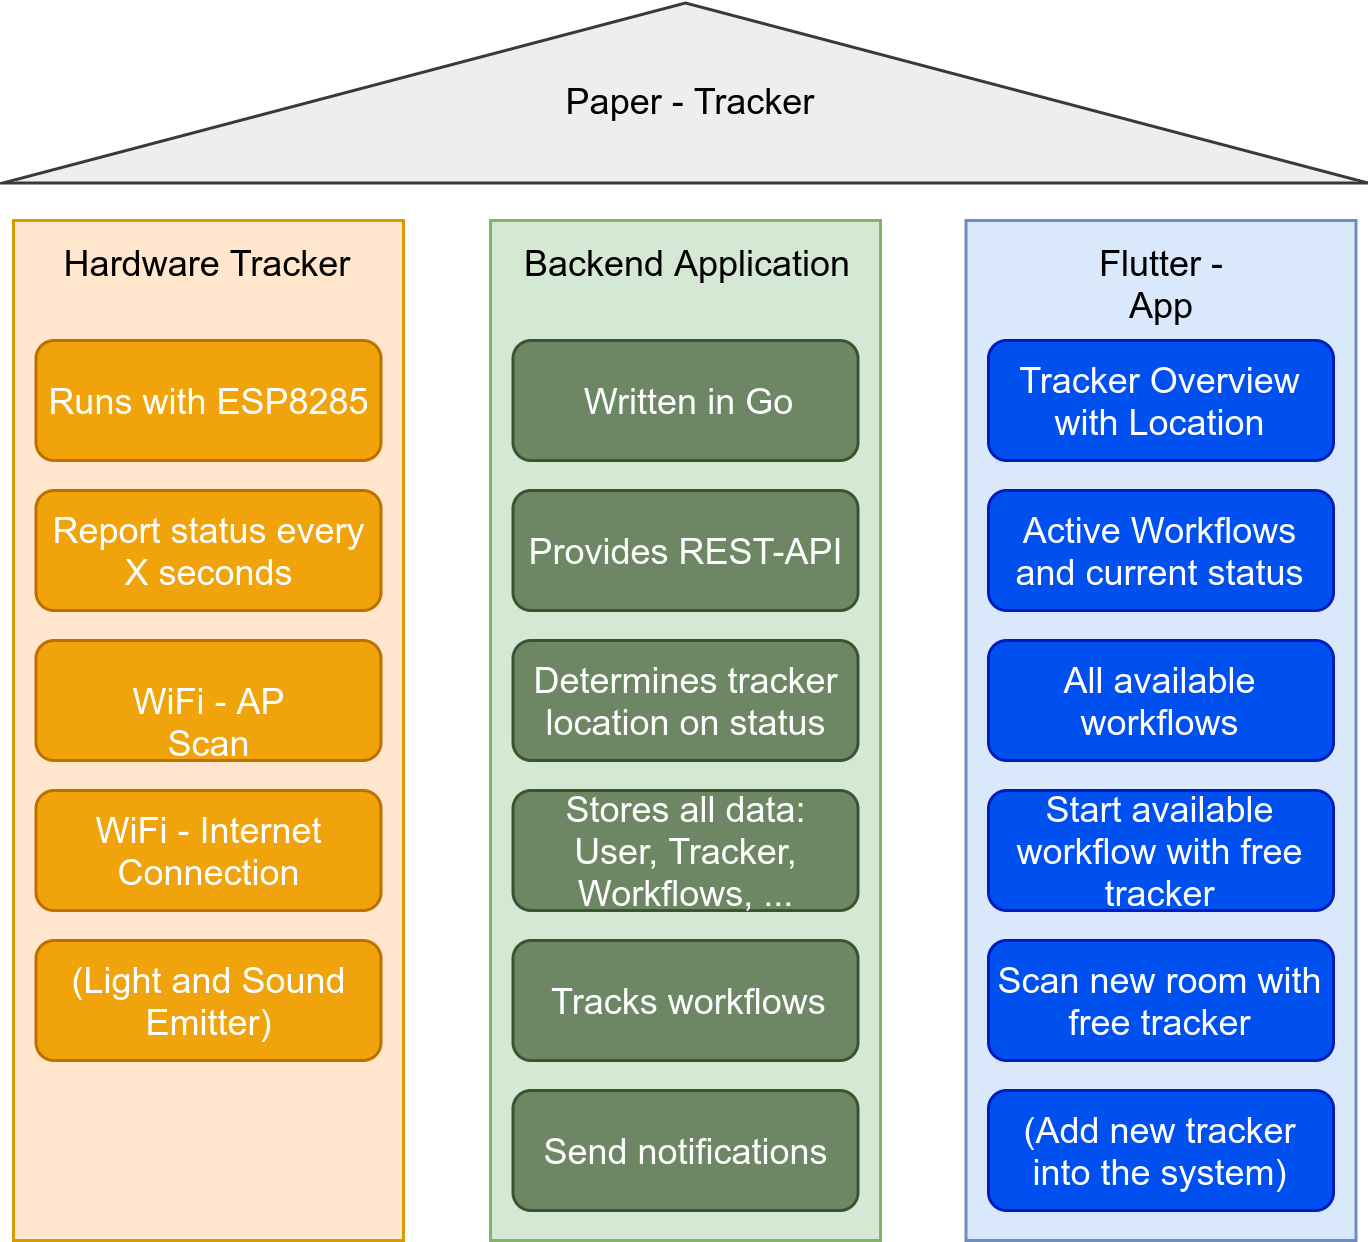
\includegraphics[width=\textwidth]{images/architecture.png} 
	\centering
	\caption{Architektur des Paper-Tracker}
	\label{fig:architecture}
\end{figure} 

\section{Komponentenarchitektur} \label{sec:komponentenarchitektur}

In den folgenden Abschnitten wird detaillierter auf die einzelnen Komponenten des in
\autoref{sec:systemarchitektur} beschriebenen Systems eingegangen.
Dabei werden die Komponenten in derselben Reihenfolge beschrieben, in welcher die Daten im
Gesamtsystem fließen.

\subsection{Tracking mit IoT-Hardware} \label{sec:tracking-hardware}

Zur Erfassung der Standortdaten der Dokumente werden, wie in \autoref{sec:soll-analyse}
beschrieben, Hardware-Tracker eingesetzt.
\TODO{Es wäre schön, Glossar-Referenzen zu kennzeichnen (oft mit Glos, oder Gls)}
Diese verwenden jedoch keine absolute Positionierungstechnologie wie beispielsweise \gls{GPS}, da
das hierfür benötigte Satellitensignal in Gebäuden zu schwach, und somit die Positionierung
fehlschlagen kann.
\TODO{Quelle für die Genauigkeit von GPS in Gebäuden}

\TODO{Ist das hier eher Analyse?}
Für die Lokalisierung von Geräten innerhalb eines Gebäudes gibt es daher mehrere Ansätze.
\TODO{Glossar: Mesh-Netzwerk}
Eine Möglichkeit ist es, ein Mesh-Netzwerk aus den Tracker-Geräten aufzubauen. Ist die Position
einiger weniger Knoten des Meshes bekannt, kann durch die Signalstärke zu umliegenden Knoten oder
über die sogenannte Time-of-Arrival bestimmt werden, wo sich ein Knoten relativ zu anderen Knoten
und damit auch zu den Knoten mit bekannter Position befindet.
\TODO{Time-of-Arrival erläutern}
Mit dieser Methode kann eine Genauigkeit von bis zu einem Meter bei der Lokalisierung erzielt
werden. (vgl. \cite{Patwari2003})

Eine weitere Möglichkeit ist, auf bestehende Infrastruktur zurückzugreifen. \Gls{WLAN} ist
heutzutage in praktisch jedem Gebäude verfügbar.
In Gebäuden, in welchen es mehrere \glspl{AP} gibt, kann die Position dadurch bestimmt werden,
dass der Tracker auswertet, von welchen \glspl{AP} er ein Signal empfängt und wie stark der
Empfang zum jeweiligen \gls{AP} ist.
Da die Positionsdaten ohnehin zur Auswertung an das Backend übertragen werden müssen, wofür eine
\gls{WLAN}-Verbindung notwendig ist, wird diese Methode eingesetzt.

Um die Daten über die Signalstärke an das Backend zu übermitteln wird das Protokoll \gls{CoAP}
eingesetzt. Hierbei handelt es sich um ein spezialisiertes Protokoll für die Verwendung in
\gls{IoT}-Hardware, welches dafür optimiert wurde möglichst wenig Overhead zu haben.
\TODO{Glossar: Overhead}
Im \gls{IoT}-Bereich haben sich einige Protokolle durchsetzen können. Dazu zählen vor allem
\gls{HTTP}, \gls{MQTT}, \gls{AMQP} und \gls{CoAP}.
Da die Tracker Batteriebetrieben sind, ist für diesen Anwendungsfall besonders die Performance des
eingesetzten Protokolles wichtig. Je weniger Overhead das Protokoll aufweist, desto weniger
Instruktionen müssen vom Prozessor des Trackers durchgeführt werden, was zu einer längeren Laufzeit
führt.
Werden die Protokolle anhand dieses Aspektes verglichen, erweist sich \gls{CoAP} als effizientestes
Protokoll. (vgl. \cite{Dizdarevic2019}, \cite{Naik2017})
\TODO{Quellen verwenden, die in diesem Paper zitiert werden}

\subsection{Backend-Anwendung} \label{sec:backend}

Da die Backend-Anwendung die zentrale Komponente des Systems ist und auch die Daten verwaltet, werden für sie die Daten-Klassen modelliert.
Das resultierende UML-Diagramm ist in Abbildung \ref{fig:uml} abgebildet.

Die zentrale Klasse des Diagramms bildet die \enquote{Tracker}-Klasse.
Sie modelliert einen Hardware-Tracker.
Als Attribut besitzt sie eine Referenz auf einen \enquote{Room}.

Ein \enquote{Room} ist ein physikalischer Raum, der von einem Tracker erkannt werden soll.
Neben einem Identifizierer und einem \enquote{Label} (Name) für den Raum werden zusätzlich mehrere \enquote{BSSIDTrackingData} gespeichert.
Diese beinhalten für einen spezifischen \enquote{Access Point} einige Messdaten zu der gemessenen Signalstärke.
Über diese kann über eine Antwort des Trackers mit \enquote{ScanResults} die Position des Tracker bestimmt werden.

Damit der Tracker eine Antwort sendet, wird diese mit Hilfe eines Kommandos angefragt.
Diese Kommandos werden jeweils in einer Instanz der \enquote{Command}-Klasse abgebildet.
Pro Tracker können somit mehrere Kommandos abgespeichert werden.
Die Kommandos besitzen einen spezifischen Typ der Enumeration \enquote{CommandType}, der die Aktion des Kommandos bestimmt.
Auch wird pro Kommando eine \enquote{SleepTimeSec} festgelegt, die bestimmt wie lange der Tracker sich abschalten darf.

Spezielle Antworten der Tracker auf Kommandos und auch des Servers auf Anfragen der App sind in dem Unterpaket \enquote{communication} modelliert.
Dies ist zum Beispiel eine Fehler-Antwort und eine Basisklasse für Antworten des Trackers.
Diese \enquote{TrackerResponse}-Klasse besitzt auch ein Feld für den aktuellen Batteriestand des Trackers, um diesen überwachen zu können. 

\begin{figure}
	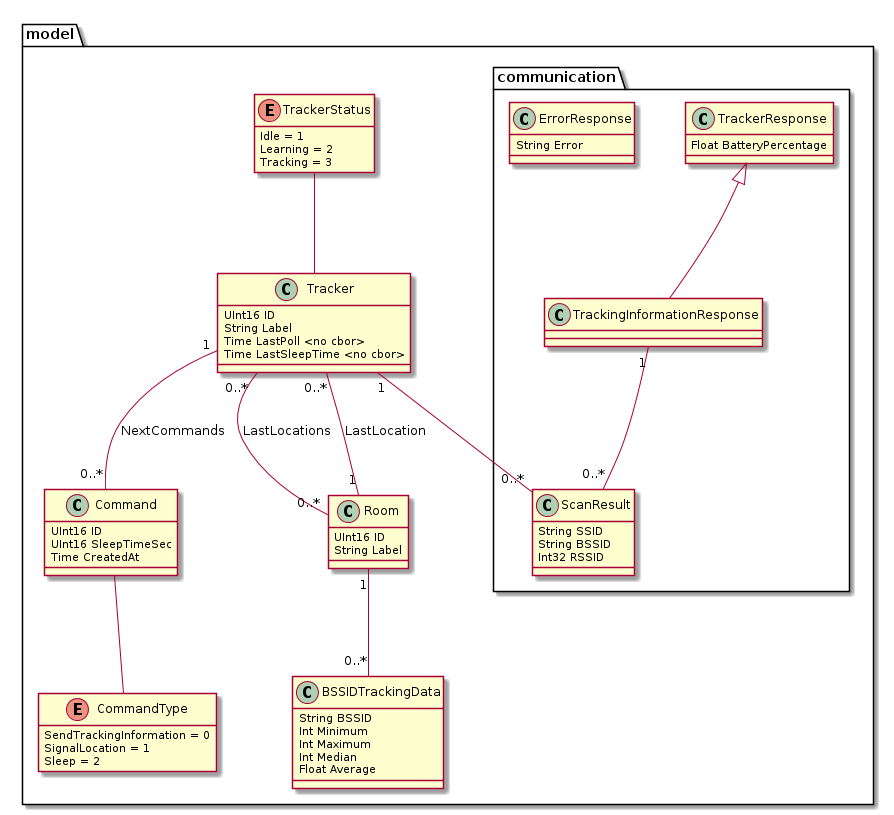
\includegraphics[width=\textwidth]{images/uml.png} 
	\centering
	\caption{UML-Diagramm für die Backend-Anwendung}
	\label{fig:uml}
\end{figure} 

\FloatBarrier
\subsection{App für Mobilgeräte} \label{sec:app}
